\documentclass[12pt]{article}

\usepackage[utf8]{inputenc}
\usepackage[margin=0.6in]{geometry}

\usepackage{amsmath}
\usepackage{graphicx}

\title{Ph 223 Problem Set 1}
\author{Alex Zahn}
\date{10/7/2016}

\begin{document}

\maketitle

\newcommand{\wmsq}{W/\(\mathrm{m}^2\,\)}
\newcommand{\msq}{\(\mathrm{m}^2\,\)}
\newcommand{\micron}{\(\mu\mathrm{m}\)\,}
\newcommand{\mcb}{\(\mathrm{m}^3\,\)}


\section{Spectrophotometric Distance Estimates of Binary Stars}

\subsection*{a}

We have a parallax angle of 768.13 mas, which corresponds to a distance of about 1.3 pc.


\section{HR Diagram}

Below we have an HR diagram generated from the theoretical values from the course website. Black points are dwarf stars, red points are giants, and blue points are supergiants. O type stars are plotted with an open circle. Lines of constant radius are shown for .2, 1, 5, 10, 50, 100, 500 and 2500 solar radii. We can see that (at least of the theoretical stars we're given) most giants are between five and fifty solar radii and most supergiants are between and twenty five hundred solar radii. I will look into annotating the graph with labels for the lines of constant radius eventually.

\begin{center}
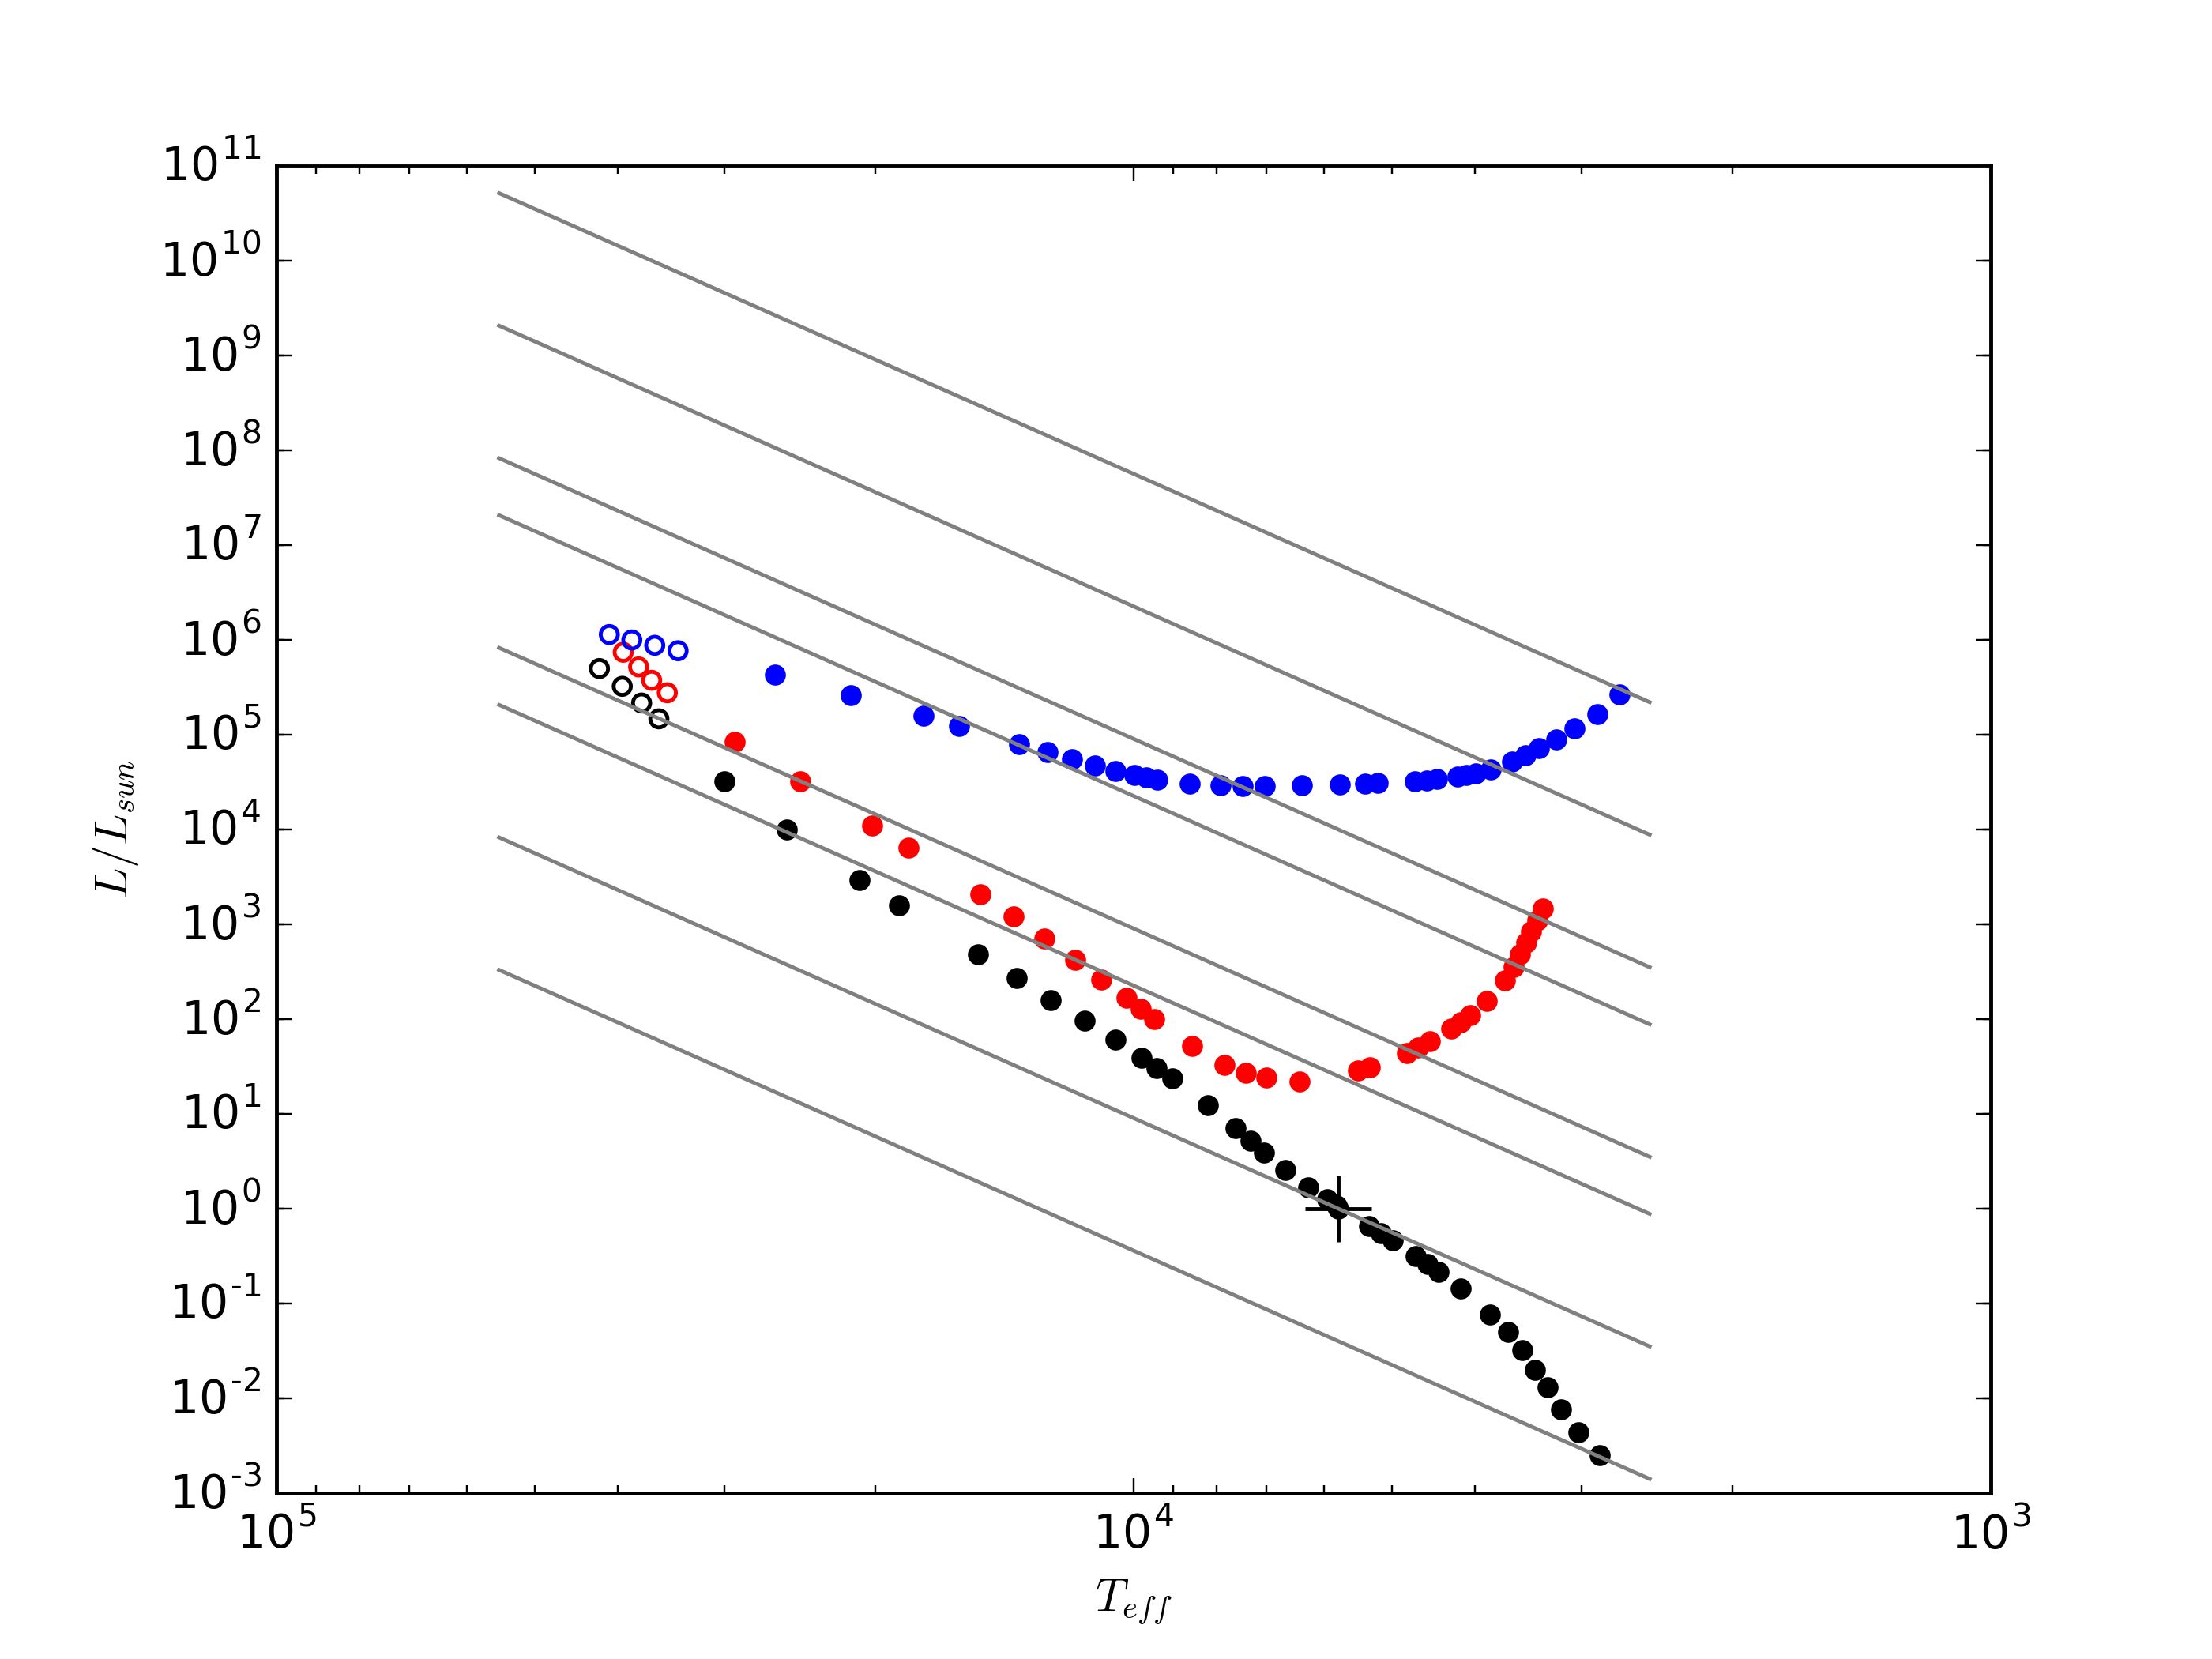
\includegraphics[scale=.7]{HR.png}
\end{center}



\section{A Simple Star Model}

\subsection*{a}

From mass continuity, \(\frac{dr}{dm} = \frac{1}{4\pi r^2 \rho}\). With our assumed density profile, this is a separable equation:

\[ \int 4\pi \rho_c r^2\left(1-\frac{r}{R}\right)dr = \int dm
\]

\(r(m=0) = 0\) so that we have

\[ 4\pi \rho_c \left( \frac{r^3}{3} - \frac{r^4}{4R} \right) = m
\]

From hydrostatic equilibrium, \(\frac{dP}{dr} = \frac{-Gm}{r^2}\rho\). We've just found \(m\) as an explicit function of \(r\), so we can integrate this for the pressure profile right away.

\begin{align*}
P &= P_c + \int_0^r \frac{dP}{dr}dr \\[12pt]
&= P_c - \int_0^r 4\pi\rho_c G \left(  \frac{r}{3} - \frac{r^2}{4R} \right)\left( \frac{1}{r^2} - \frac{1}{Rr} \right)dr \\[12pt]
&= P_c - \frac{1}{36R^2} \pi\rho_c G r^2\left( 9r^2 -28Rr + 24R^2 \right)
\end{align*}

So the surface pressure \( P_s \equiv P(R)\) is \(P_c - \frac{5}{36}\pi\rho_c G R^2\). One hopes that \(P_s \ll P_c\), in which case \(P_c \approx \frac{5}{36}\pi\rho_cG R^2\). From the form we already have for \(m\), \(M = m(R) = \frac{1}{3}\pi\rho_c R^3 \) so that we can write

\[ P_c \approx \frac{5}{4\pi\rho_c}G\frac{M^2}{R^4}
\]

although the dependence isn't really \(M^2/R^4\) since we know \(\rho_c = 3M/\pi R^3\). A better expression is

\[ P_c = \frac{5GM}{12R}\]

\subsection*{b}

First, we need an expression for the number density. 

\section{MESA}

Looks like MESA is running on my lab machine, and that the tutorial runs evolve the star to sixty thousand and and ten million years:

\begin{center}
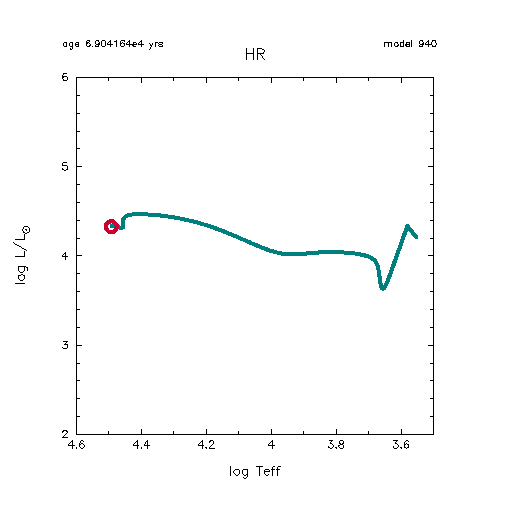
\includegraphics[scale=.7]{HR_pre.png}
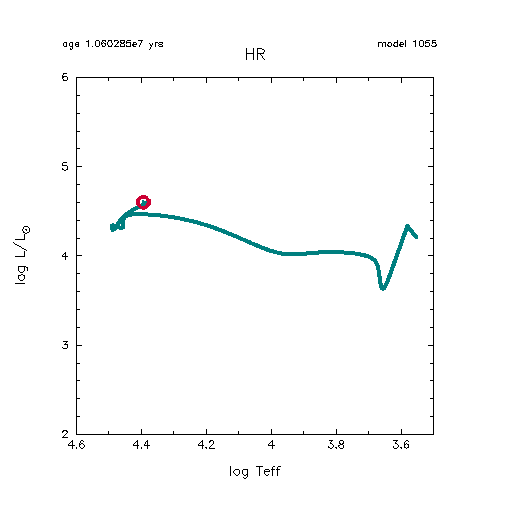
\includegraphics[scale=.7]{HR_post.png}
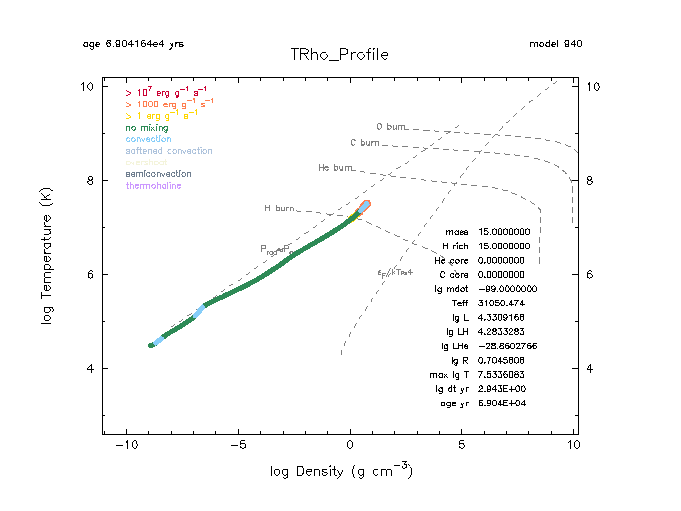
\includegraphics[scale=.6]{trho_pre.png}
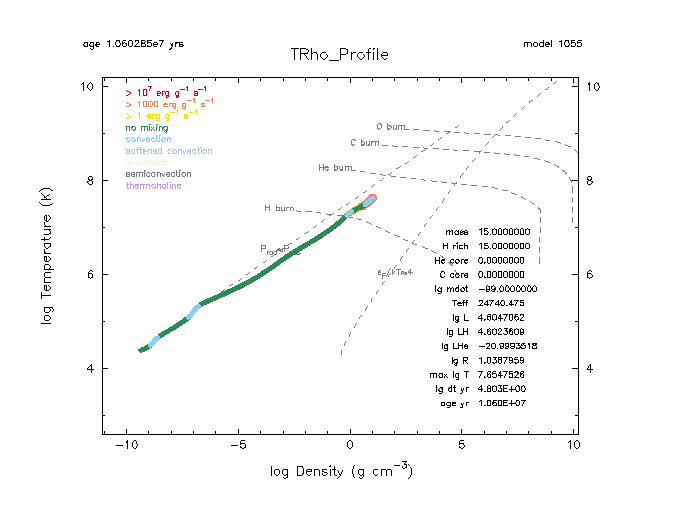
\includegraphics[scale=.6]{trho_post.png}
\end{center}



\end{document}